\documentclass[a4paper]{article}

% ===== Packages =====
\usepackage[T1]{fontenc}        % Font encoding
\usepackage{lmodern}
\usepackage{algorithm}
\usepackage{subcaption}

% Modern font
\usepackage[a4paper,margin=0.8in]{geometry} % Page layout: 1in margin
\usepackage[fleqn]{amsmath}     % Math symbols, left-aligned equations
\setlength{\mathindent}{0pt}    % No indent for fleqn
\usepackage{amssymb}            % Extra math symbols
\usepackage{booktabs}           % Better tables
\usepackage{graphicx}           % Include graphics
\usepackage{setspace}           % Adjust line spacing
\usepackage{titling}            % Customize title format
\usepackage{float}              % [H] for figure placement
\usepackage{color}              % For colored text
\usepackage{booktabs}           % For better tables
\usepackage[colorlinks=true, linkcolor=blue, citecolor=blue, urlcolor=blue]{hyperref}
\usepackage{algorithm}
\usepackage{algorithmic}
\renewcommand{\thealgorithm}{\arabic{algorithm}} % Numerazione autonoma

\newcommand{\todo}[1]{\textcolor{red}{\textbf{TODO:} #1}}

% ===== Line spacing =====
\setstretch{0.9}                % 0.9× spacing; regola a piacere

% ===== Title formatting =====
\pretitle{%
  \begin{center}\bfseries\Large
  }
  \posttitle{%
  \end{center}\vspace{-1em}
}
\preauthor{%
  \begin{center}\small
  }
  \postauthor{%
  \end{center}\vspace{-1em}
}
\predate{}  % no date before
\postdate{} % no date after

% ===== Metadata =====
\title{Report HW3}
\author{%
  \ifdefined\anonymous%
  Anonymous Submission
  \else
  \begin{tabular}{cc}
    Simone De Carli & Damiano Salvaterra \\
    {\small\texttt{simone.decarli@studenti.unitn.it}} &
    {\small\texttt{damiano.salvaterra@studenti.unitn.it}}
  \end{tabular}
  \fi
}
\date{}  % leave date blank

\begin{document}

\maketitle

\section*{Exercise 1}

Given a dataset of approximately $3\cdot 10^4$ entries of the form $(x,y)$, where $x$ is a time value and $y$ is its corresponding value, we are interested in modeling the statistics of the dataset. There is a clear trend in the data.

\subsection*{Part 1: Visualize the trend}

First, we need to visualize the trend in the data. To do this, we scatter plot the data points (\ref{fig:trend-scatter}) and we plot the distribution of the data points (\ref{fig:trend-hist}) that we cannot trust.

\begin{figure}[htbp]
  \centering
  \begin{subfigure}[t]{0.4\textwidth}
    \centering
    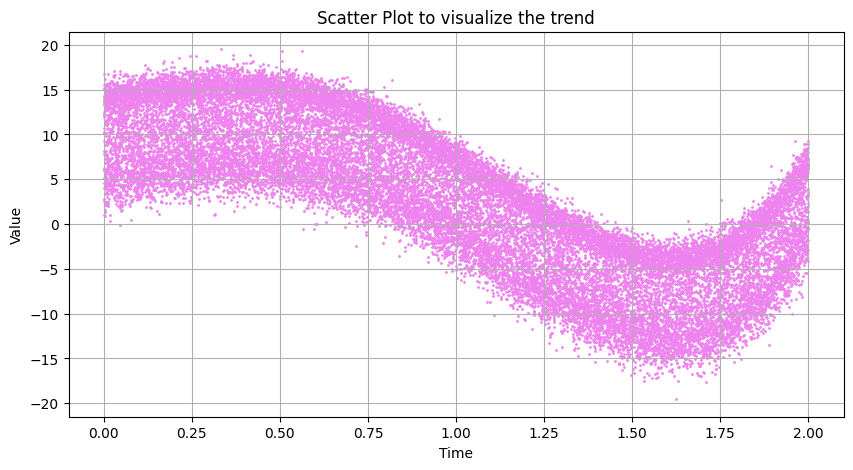
\includegraphics[width=\textwidth]{images/trended_scatter.png}
    \caption{Scatter plot of the dataset.}\label{fig:trend-scatter}
  \end{subfigure}
  \hfill
  \begin{subfigure}[t]{0.4\textwidth}
    \centering
    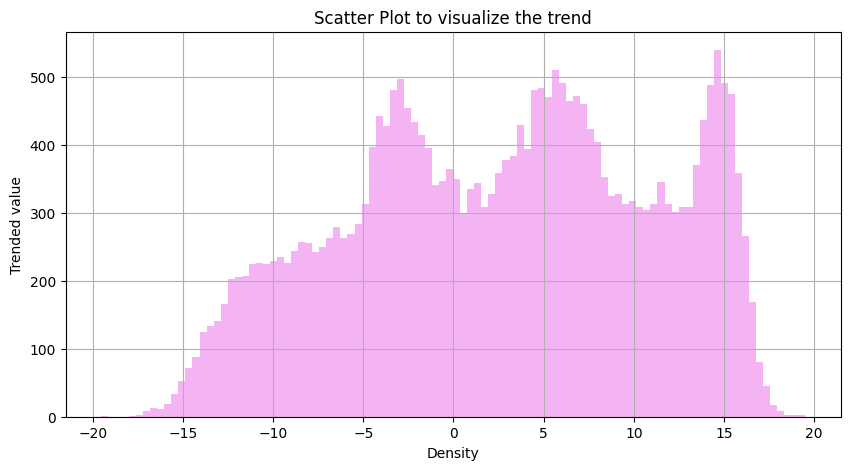
\includegraphics[width=\textwidth]{images/trended_dist.png}
    \caption{Histogram of the dataset.}\label{fig:trend-hist}
  \end{subfigure}
  \caption{Trended dataset.}\label{fig:trend}
\end{figure}

\subsection*{Part 2: Fit a polynomial trend}

We estimate a polynomial trend using the least squares method for degrees from 1 to 8 (\ref{fig:poly-trend}).

\begin{figure}[htbp]
  \centering
  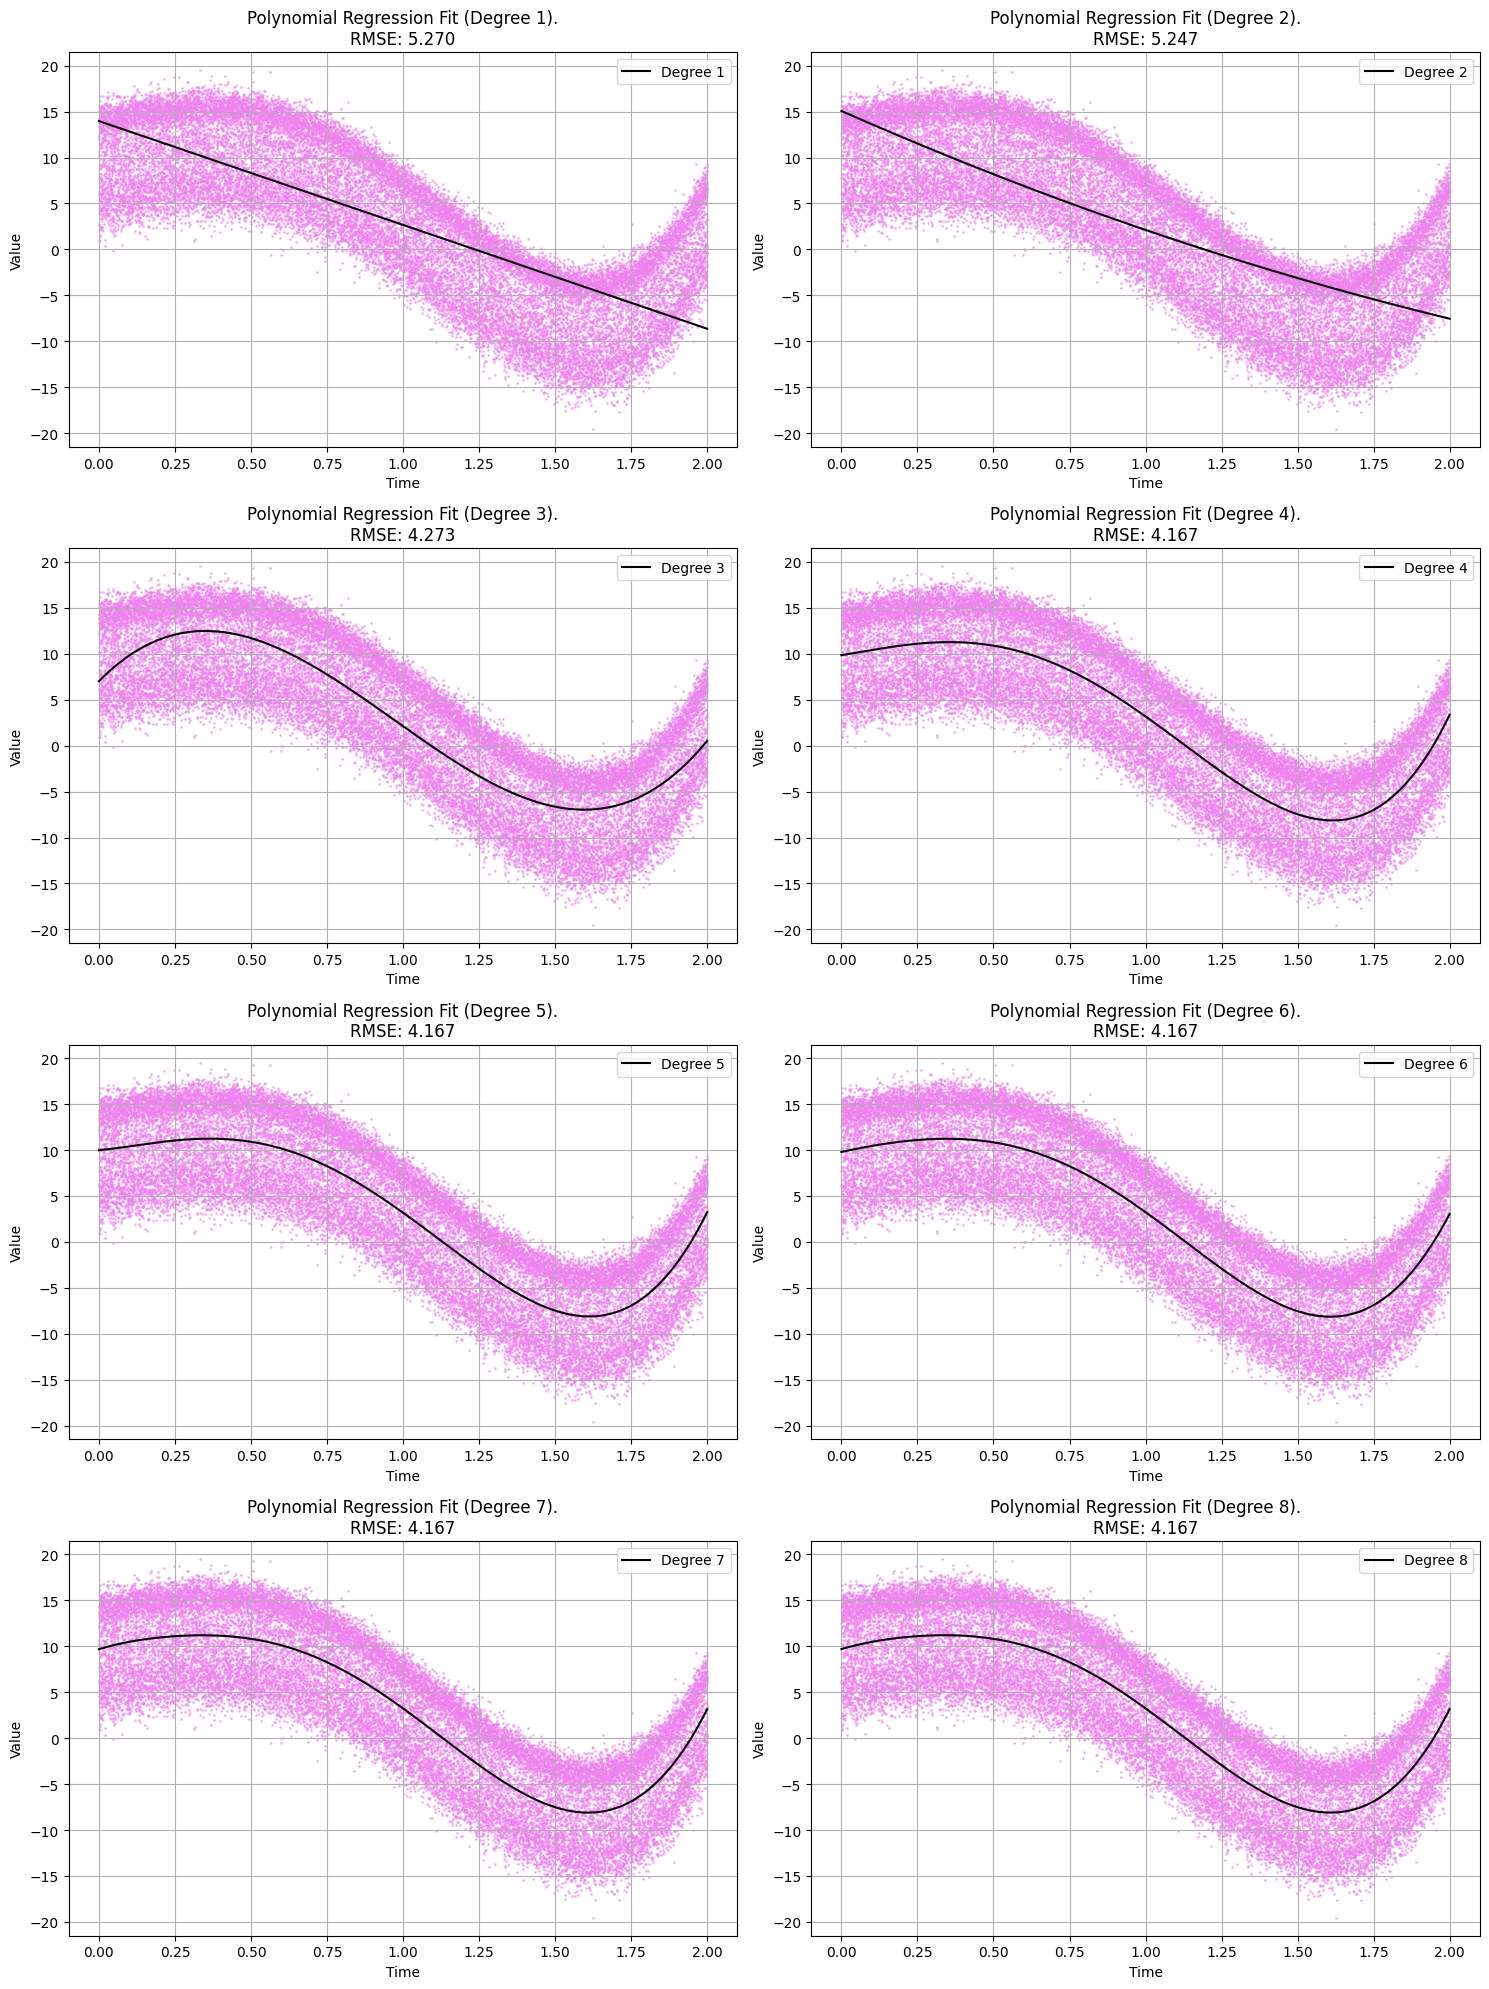
\includegraphics[width=\textwidth]{images/poly_trends.png}\caption{
    Polynomial trends fitted to the dataset.
  }\label{fig:poly-trend}
\end{figure}

\subsection*{Part 3: Find the best degree and remove the trend}

To remove the trend, we need to decide which polynomial degree is the best. Then we can de-trend the data.

\subsubsection*{Find the best degree}

To decide which polynomial degree is the best, we use the root mean square error (RMSE) of the polynomial fit for each degree (\ref{fig:rmse}). We also use cross-validation to estimate the RMSE of the polynomial fit for each degree (\ref{fig:cv-rmse}).

Both methods in Figure~\ref{fig:degrees} show that the best degree is 4.

\begin{figure}[htbp]
  \centering
  \begin{subfigure}[t]{0.4\textwidth}
    \centering
    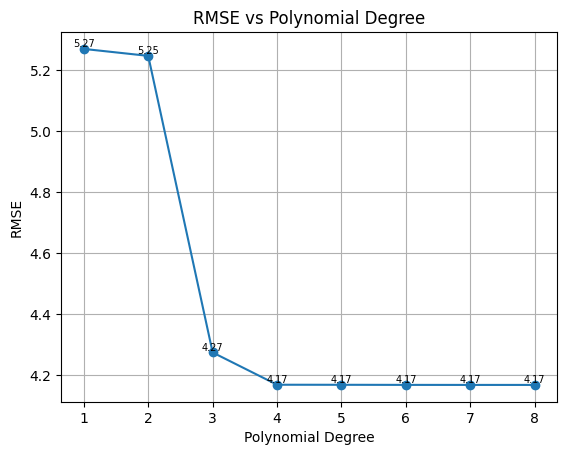
\includegraphics[width=\textwidth]{images/degrees_rmse.png}
    \caption{
      RMSE of the polynomial for each degree.
    }\label{fig:rmse}
  \end{subfigure}
  \hfill
  \begin{subfigure}[t]{0.4\textwidth}
    \centering
    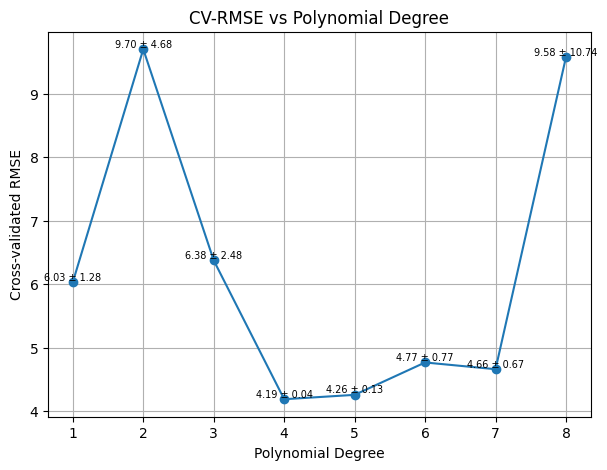
\includegraphics[width=\textwidth]{images/cv_degrees_rmse.png}
    \caption{
      Mean RMSE from the cross-validation for each degree.
    }\label{fig:cv-rmse}
  \end{subfigure}
  \caption{
    Evaluation of the polynomial degree.
  }\label{fig:degrees}
\end{figure}

\subsubsection*{De-trend the data}

To de-trend the data, we just subtract the best polynomial fit (degree 4) from the data. The result is shown in Figure~\ref{fig:detrended}.

\begin{figure}[htbp]
  \centering
  \begin{subfigure}[t]{0.4\textwidth}
    \centering
    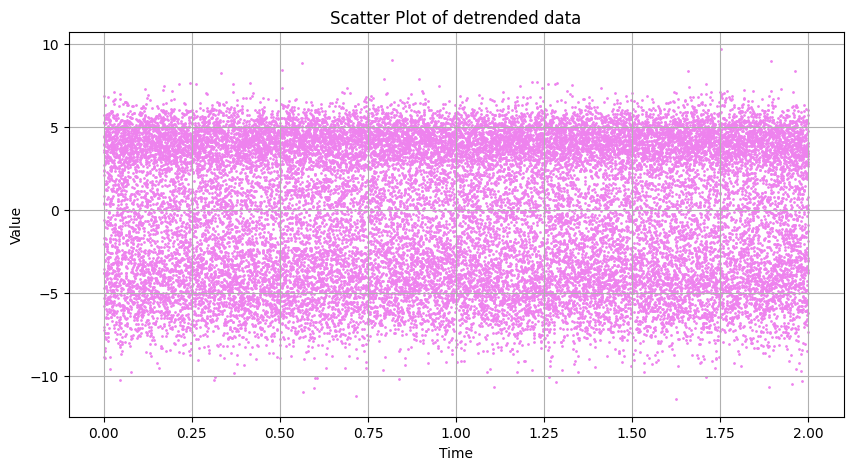
\includegraphics[width=\textwidth]{images/detrended_scatter.png}
    \caption{
      Scatter plot of the de-trended dataset.
    }\label{fig:detrended-scatter}
  \end{subfigure}
  \hfill
  \begin{subfigure}[t]{0.4\textwidth}
    \centering
    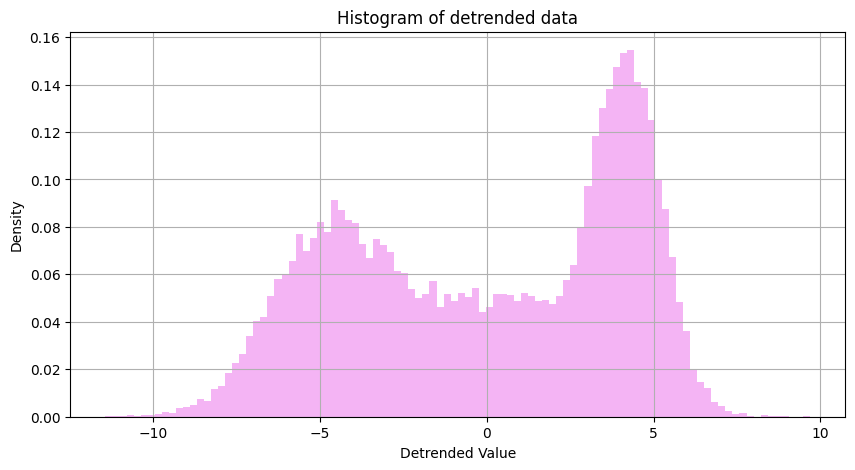
\includegraphics[width=\textwidth]{images/detrended_dist.png}
    \caption{
      Histogram of the de-trended dataset.
    }\label{fig:detrended-hist}
  \end{subfigure}
  \caption{
    De-trended dataset.
  }\label{fig:detrended}
\end{figure}

\subsection*{Part 4: Fit a mixture of Gaussians}

To fit a mixture of Gaussians to the de-trended data, we implement the EM algorithm.

We run the EM algorithm with a maximum of $10^3$ iterations and a tolerance of $10^{-6}$ with two initilization settings:
\begin{itemize}
    \setlength\itemsep{0.01em}
  \item starting from a uniform prior, means randomly chosen from the data, and variances all equals to the dataset variance;
  \item starting from K-means clustering parameters, i.e.~setting the priors as the fraction of points for each cluster, means as the cluster centroids and variances estimated as intra-cluster variances.
\end{itemize}

The results of the EM algorithm are shown in Table~\ref{tab:gmm-results} and visualized in Figure~\ref{fig:gmm-plot}.

\begin{table}[htbp]
  \centering
  \small
  \begin{tabular}{l cc|ccc|ccc}
    \toprule
    & \multicolumn{2}{c}{Original} & \multicolumn{3}{c}{KMeans init (iter.\ 569)} & \multicolumn{3}{c}{Random init (iter.\ 473)} \\
    \cmidrule(lr){2-3} \cmidrule(lr){4-6} \cmidrule(lr){7-9}
    Component & $\mu$ & $\sigma^2$ & Weight & $\mu$ & $\sigma^2$ & Weight & $\mu$ & $\sigma^2$ \\
    \midrule
    1 &  -5 & 3 & 0.3443 & -4.7274 & 3.0625 & 0.3443 & -4.7274 & 3.0625 \\
    2 &  0 & 6 & 0.3024 & 0.4021 & 5.9683 & 0.3534 & 0.4021 & 5.9683 \\
    3 & 4 & 1 & 0.3534 & 4.2616 & 0.9841 & 0.3534 & 4.2616 & 0.9841 \\
    \bottomrule
  \end{tabular}
  \caption{
    Results from the EM algorithm for the two initialization settings compared to the original Gaussian parameters.
  }\label{tab:gmm-results}
\end{table}

\begin{figure}[htbp]
  \centering
  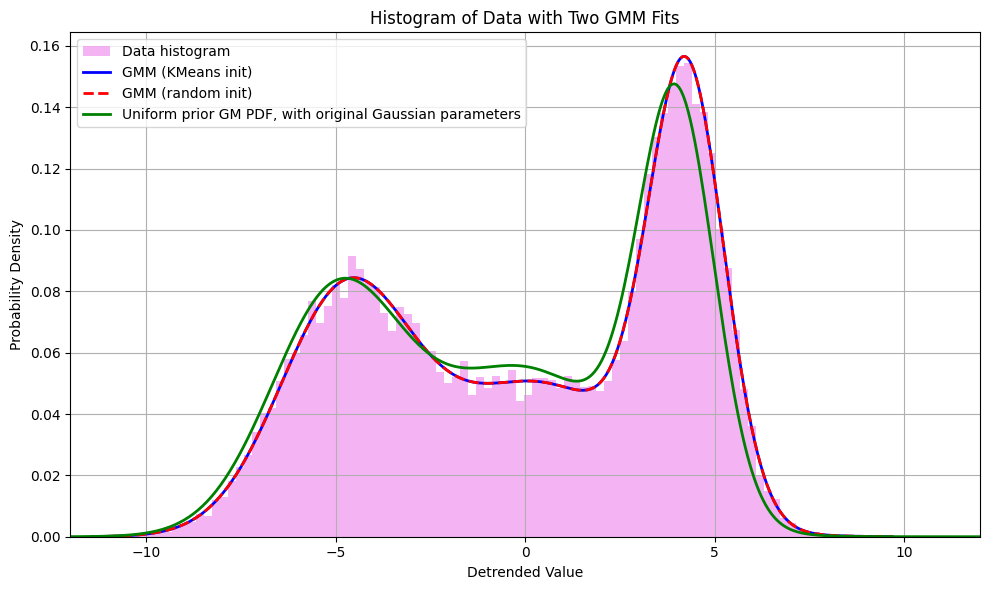
\includegraphics[width=0.6\textwidth]{images/gmm.png}\caption{
    Gaussian Mixture Models fitted to the de-trended distribution in comparison with the original gaussians assuming uniform priors.
  }\label{fig:gmm-plot}
\end{figure}

\subsection*{Part 5: Find the optimal number of gaussians}

To find the optimal number of Gaussians, we use the Bayesian Information Criterion (BIC) as regularization term. The BIC is defined as:
\begin{equation}
  \text{BIC} = -2\log L + k\log n
\end{equation}
where $L$ is the likelihood of the model, $k$ is the number of parameters in the model, and $n$ is the number of data points.
The BIC is a trade-off between the goodness of fit of the model and the complexity of the model that aims to avoid overfitting.

We fit GMM models with 1 to 10 Gaussians for a maximum of $10^3$ iterations and a tolerance of $10^{-6}$ with random means initialization as before.
The BIC scores are shown in Figure~\ref{fig:gmm-eval} and the optimal number of Gaussians is 3.

\begin{figure}[htbp]
  \centering
  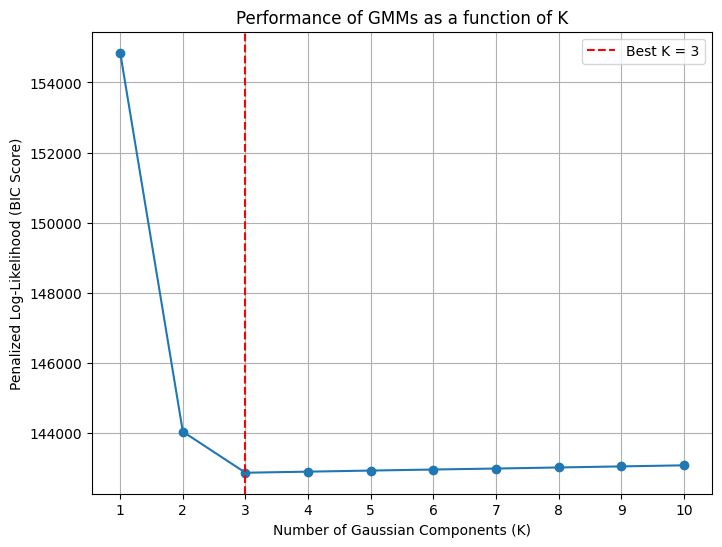
\includegraphics[width=0.4\textwidth]{images/gmms-eval.png}\caption{
    Bayesian Information Criterion (BIC) score for increasing number of gaussians.
  }\label{fig:gmm-eval}
\end{figure}

\end{document}
